\documentclass[twoside]{article}
\usepackage{amsmath,amssymb,amsthm,graphicx}
\usepackage{epsfig}
\usepackage[authoryear]{natbib}
\bibliographystyle{unsrtnat}
\usepackage{geometry}
\usepackage{setspace}

\geometry{twoside,
          letterpaper, % i.e, paperwidth=210mm and paperheight=297mm,
          top=25mm,
          bottom=45mm,
          left=25mm,
          right=25mm,
}

\setlength{\parindent}{0pt}
\setlength{\parskip}{0.5cm}
% Local Macros Put your favorite macros here that don't appear in
% stat-macros.tex.  We can eventually incorporate them into
% stat-macros.tex if they're of general use.

\begin{document}

\textbf{Reflection - Gaussian Process - Rasmussen, Williams}\\
\textbf{Nicholas Hoernle \hfill \today}

\begin{enumerate}
  \item As the predictive input ($x_*$) gets further from the training data ($\mathbf{x}$), in this case the 5 points that are plotted), the co-variance between any one data point in $\mathbf{x}$ and the predictive input $x_*$ tends to 0 since $k(x_p, x_q) = \exp \{ -\frac{1}{2} \vert x_p - x_q \vert ^2 \} \rightarrow 0$ as $\vert x_p - x_q \vert$ gets large. Therefore, as we extend the horizontal axis to -100, the data plays no role in the posterior and the posterior is essentially equal to the prior. In this case, the prior is given in Fig 2.2 a and therefore we expect the posterior at points far from the training data to be very similar to the prior (for both the draws and the gray co-variance that is plotted). Fig~\ref{problem_distribution} shows a slightly extended boundary to the left but the plot clearly resembles the prior for $x < -8$.
  \item In regression, prediction is assigning an expected value and covariance to data for which we do not have training examples. In Fig 2.2 b., we see the gray area as the covariance around a predicted mean (not shown) for all values of $x_* \in [-5,5]$ (in practice, the authors only make the predictions for a discrete set of 100 points and not for the continuous values as the plot implies).
  \item The content is from \textit{Prediction with Noise-free Observations}. The co-variance shrinks to $0$ around the observed data, thus we assume these data are noise-free observations.
\end{enumerate}

\begin{figure}[h]
\centering
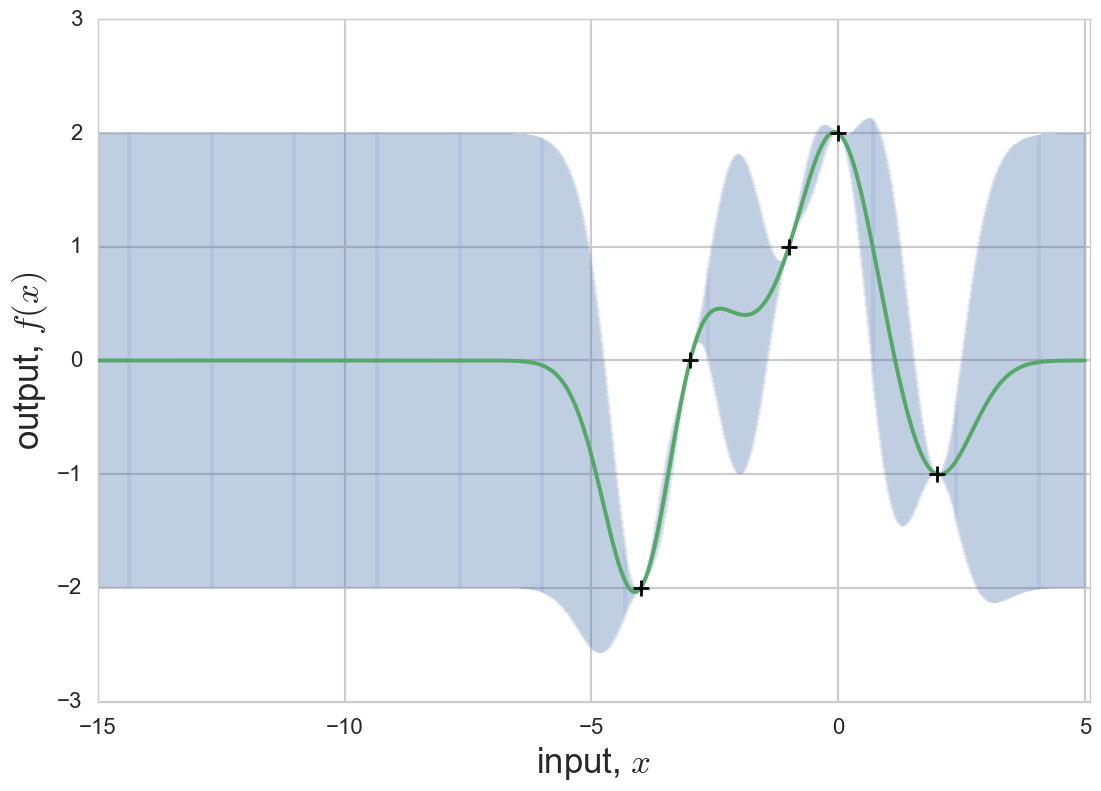
\includegraphics[width=6cm]{fig2_2breplication.png}
\caption{Replicated Fig 2.2b with left boundary extended to see that the prior dominates as we move away from the data.}\label{problem_distribution}
\end{figure}


% \bibliography{references}

\end{document}
